\documentclass[a4paper, 12pt]{article}

\input{/home/nick/latex-preambles/xelatex.tex}

\setmainfont{Minion Pro}

\newcommand{\imagesPath}{.}

\title{
	\textbf{Εργαστήριο Δικτύων Υπολογιστών} \\~\\
	Εργαστηριακή Άσκηση 2 \\ 
	Δικτύωση συστημάτων στο VirtualBox
}
\author{}
\date{}

\begin{document}
	\maketitle
	\begin{center}
	\begin{tabular}{|l|l|}
		\hline
		\textbf{Ονοματεπώνυμο:} Νικόλαος Παγώνας, el18175  & \textbf{Όνομα PC:} nick-ubuntu \\
		\hline
		\textbf{Ομάδα:} 1 (Τρίτη 10:45) & \textbf{Ημερομηνία Εξέτασης:} Τρίτη 08/03/2022 \\
		\hline
	\end{tabular}
	\end{center}

\section*{Άσκηση 1 (προετοιμασία): Δημιουργία εικονικού FreeBSD}

	\subsection*{1.1}
		Επισκεπτόμαστε την ιστοσελίδα της εκφώνησης και εντοπίζουμε τα VM images για επεξεργαστές \verb|i386|.
	
	\subsection*{1.2}
		Κατεβάζουμε το αντίστοιχο αρχείο και το αποσυμπιέζουμε.

	\subsection*{1.3}
		Δημιουργούμε ένα νέο εικονικό μηχάνημα στο VirtualBox με τα ζητούμενα χαρακτηριστικά.

	\subsection*{1.4}
		Από το γραφικό περιβάλλον του VirtualBox αλλάζουμε τις ζητούμενες παραμέτρους για μνήμη γραφικών, USB και Network.

	\subsection*{1.5}
		Ξεκινάμε το εικονικό μηχάνημα και κάνουμε login ως root.

	\subsection*{1.6}
		Με τη βοήθεια της εντολής \verb|passwd| ορίζουμε συνθηματικό \verb|ntua| για τον root.

	\subsection*{1.7}
		Με τη βοήθεια της εντολής \verb|adduser| δημιουργούμε έναν νέο χρήστη \verb|lab| που έχει τα ζητούμενα χαρακτηριστικά.

	\subsection*{1.8}
		Στο αρχείο \verb|/etc/rc.conf| προσθέτουμε τις ζητούμενες γραμμές, διαγράφοντας ό,τι υπάρχει.

	\subsection*{1.9}
		Δημιουργούμε το αρχείο \verb|/boot/loader.conf|, το οποίο περιέχει τη ζητούμενη εντολή για επιτάχυνση της διαδικασίας εκκίνησης.

	\subsection*{1.10}
		Επανεκκινούμε το FreeBSD χωρίς προβλήματα και με την εντολή \verb+service -e | grep sshd+ βεβαιωνόμαστε ότι η υπηρεσία \verb|sshd| τρέχει.

	\subsection*{1.11}
		Διαγράφουμε το ιστορικό των εντολών που δώσαμε μέχρι το σημείο αυτό με την εντολή \verb|history -c|. 

	\subsection*{1.12}
		Διαγράφουμε όποιο αρχείο \verb|/var/db/dhclient.leases.*| έχει δημιουργηθεί κατά την εκκίνηση με την εντολή \verb|rm /var/db/dhclient.leases.*|.

	\subsection*{1.13}
		Κλείνουμε το εικονικό μηχάνημα με την εντολή \verb|poweroff|.

	\subsection*{1.14}
		Από τη διαδρομή File$\rightarrow$Export Appliance... δημιουργούμε ένα αρχείο \verb|FreeBSD11.4.ova|.

	\subsection*{1.15}
		Αποθηκεύουμε το αρχείο \verb|.ova| για μελλοντική χρήση και διαγράφουμε το αρχείο \verb|.vhd|, αφού δεν χρειάζεται πλέον.
	
\section*{Άσκηση 2: Ανάλυση δικτυακών πρωτοκόλλων με το TCPDUMP}

	\subsection*{2.1}
		Με την εντολή \verb|ifconfig|.

	\subsection*{2.2}
		Με τις εντολές \verb|ifconfig em0 down| και ύστερα \verb|ifconfig em0 up|.

	\subsection*{2.3}
		Με τις εντολές \verb|man tcpdump|, \verb|man pcap| και \verb|man pcap-filter|.

	\subsection*{2.4}
		Η σύνταξη είναι: \verb|tcpdump -i em0 -n|.

	\subsection*{2.5}
		Η σύνταξη είναι: \verb|tcpdump -i em0 -X|.

	\subsection*{2.6}
		Η σύνταξη είναι: \verb|tcpdump -e|.
		
	\subsection*{2.7}
		Η σύνταξη είναι: \verb|tcpdump -i em0 -s 68|.

	\subsection*{2.8}
		Η σύνταξη είναι: \\
		\verb|tcpdump -v "ip && host 10.0.0.1"| ή \verb+tcpdump -v "ip && (src or dst 10.0.0.1)"+.

	\subsection*{2.9}
		Η σύνταξη είναι: \\
		\verb+tcpdump -i em0 "(src 10.0.0.1 && dst 10.0.0.2) || (src 10.0.0.2 && dst 10.0.0.1)"+.

	\subsection*{2.10}
		Η σύνταξη είναι: \verb|tcpdump -x "ip && net 1.1.0.0/16"|.

	\subsection*{2.11}
		Η σύνταξη είναι: \verb|tcpdump -e -x "ip && (!net 192.168.1.0/24)"|.

	\subsection*{2.12}
		Η σύνταξη είναι: \verb|tcpdump "ip && broadcast"|.

	\subsection*{2.13}
		Η σύνταξη είναι: \verb|tcpdump "ip[2:2] > 576"|.

	\subsection*{2.14}
		Η σύνταξη είναι: \verb|tcpdump "ip[8:1] < 5"|.

	\subsection*{2.15}
		Η σύνταξη είναι: \verb|tcpdump "ip[0:1] & 0x0f > 5|.

	\subsection*{2.16}
		Η σύνταξη είναι: \verb|tcpdump "icmp && (src 10.0.0.1)"|.

	\subsection*{2.17}
		Η σύνταξη είναι: \verb|tcpdump "tcp && (dst 10.0.0.2)"|.

	\subsection*{2.18}
		Η σύνταξη είναι: \verb|tcpdump "udp && (dst port 53)"|.

	\subsection*{2.19}
		Η σύνταξη είναι: \verb|tcpdump "tcp && (src or dst 10.0.0.10)"|.

	\subsection*{2.20} 
		Η τροποποιημένη σύνταξη είναι: \\ \verb|tcpdump -w sample_capture "tcp && (src or dst 10.0.0.10) && (dst port 23)"|.

	\subsection*{2.21}
		Η σύνταξη είναι: \verb|tcpdump "tcp[13:1] & 0xff == 2"|.

	\subsection*{2.22}
		Η σύνταξη είναι: \verb+tcpdump "tcp[13:1] & 0xff == 2 || tcp[13:1] & 0xff == 18"+.
		
	\subsection*{2.23}
		Η σύνταξη είναι: \verb|tcpdump "tcp[13:1] & 0xff == 17"|.
		
	\subsection*{2.24}
		Η παράσταση αυτή απομονώνει την τιμή του Data Offset, και λόγω τις δεξιάς ολίσθησης κατά 2 θέσεις μας δίνει τελικά το μέγεθος του TCP Header μετρημένο σε bytes.

	\subsection*{2.25}
		Η σύνταξη είναι: \verb|tcpdump "((tcp[12:1] & 0xf0) >> 2) > 20"|.	

	\subsection*{2.26}
		Η σύνταξη είναι: \verb|tcpdump -A "port 80"|.
		
	\subsection*{2.27}
		Η σύνταξη είναι: \verb|tcpdump "dst edu-dy.cn.ntua.gr && dst port 23"|.
			
	\subsection*{2.28}
		Η σύνταξη είναι: \verb|tcpdump "ip6"|.
			

\section*{Άσκηση 3: Δικτύωση Host-only}

	\subsection*{3.1}
		Από τη διαδρομή: "File$\rightarrow$Host Network Manager$\rightarrow$Adapter" βρίσκουμε ότι η IPv4 διεύθυνση του Host-only Ethernet adapter είναι \verb|192.168.56.1|.

	\subsection*{3.2}
		Από τη διαδρομή "File$\rightarrow$Host Network Manager$\rightarrow$DHCP Server" βρίσκουμε ότι η IPv4 διεύθυνση του DHCP Server είναι \verb|192.168.56.100|, ενώ η περιοχή διευθύνσεων που μπορεί να εκχωρήσει είναι \verb|192.168.56.101-192.168.56.254|.

	\subsection*{3.3}
		Με την εντολή \verb|dhclient em0| αποδίδουμε διευθύνσεις μέσω DHCP στα εικονικά μηχανήματα.  

	\subsection*{3.4}
		Στο PC1 αποδόθηκε η διεύθυνση \verb|192.168.56.102|, ενώ στο PC2 αποδόθηκε η διεύθυνση \verb|192.168.56.103|.

	\subsection*{3.5}
		Θα εκτελέσουμε \verb|ping 192.168.56.102| από το PC2 ή \verb|ping 192.168.56.103| από το PC1. \\
		
		Εναλλακτικά για να έχουμε καλύτερη εποπτεία της επικοινωνίας θα μπορούσαμε να τρέξουμε και \verb|nc -l <port>| από το ένα μηχάνημα (πχ το PC1), και από το άλλο να τρέξουμε \verb|nc <PC1 ip> <port>|, όπου \verb|port > 1024|. Ύστερα γράφουμε ένα μήνυμα (πχ hello) και πατάμε <enter> σε οποιαδήποτε από τις δύο κονσόλες. Το μήνυμα θα πρέπει να μεταφέρεται αυτούσιο στην κονσόλα του άλλου vm.  

	\subsection*{3.6}
		Θα εκτελέσουμε \verb|ping 192.168.56.102| ή \verb|ping 192.168.56.103| από το φιλοξενούν μηχάνημα. \\
		
		Εναλλακτικά μπορούμε να ακολουθήσουμε την ίδια διαδικασία με το \verb|nc| που περιγράψαμε παραπάνω.

	\subsection*{3.7}
		Η σύνταξη της εντολής που δείχνει την προεπιλεγμένη πύλη είναι \verb|netstat -rn|.

	\subsection*{3.8}
		Όχι, δεν υπάρχει προεπιλεγμένη πύλη, αφού έχουμε Host-only networking, οπότε δεν υπάρχει επικοινωνία με εξωτερικά δίκτυα, αλλά μόνο με μηχανήματα που υπάρχουν στο εσωτερικό δίκτυο (συμπεριλαμβανομένου του host).

	\subsection*{3.9}
		Όχι, δεν μπορούμε να κάνουμε ping στην φυσική κάρτα δικτύου του φιλοξενούντος μηχανήματος, αφού έχουμε λειτουργία Host-only networking και η φυσική κάρτα δικτύου θεωρείται ότι ανήκει σε εξωτερικό δίκτυο.

	\subsection*{3.10}
		Το όνομα των μηχανημάτων όπως το αντιλαμβάνεται το λειτουργικό τους σύστημα είναι \verb|PC.ntua.lab|, το οποίο βρέθηκε με την εντολή \verb|hostname|.

	\subsection*{3.11}
		Με την εντολή \verb|hostname PC1| και την εντολή \verb|hostname PC2| μετονομάζουμε τα εικονικά μηχανήματα σε \verb|PC1| και \verb|PC2| αντίστοιχα.
		

	\subsection*{3.12}
		Με το που κάνουμε logout εμφανίζεται το εξής μήνυμα στον PC1 και τον PC2 αντίστοιχα, χωρίς εμείς να εκτελέσουμε κάποια επιπλέον εντολή:
		
		\begin{figure}[H]
			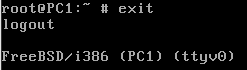
\includegraphics[width=0.5\linewidth]{\imagesPath/3.12a.png}
			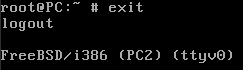
\includegraphics[width=0.5\linewidth]{\imagesPath/3.12b.png}		
		\end{figure}		
		
		Σε κάθε μηχάνημα, το νέο όνομα που αποδώσαμε φαίνεται στην παρένθεση.
		
		Αφού κάνουμε login, αυτό φαίνεται και στο prompt: 
		\begin{verbatim}
			root@PC1:~ #
		\end{verbatim} 
		\begin{verbatim}
			root@PC2:~ #
		\end{verbatim}

	\subsection*{3.13}
		Το \verb|/etc/rc.conf| στο PC1 δεν περιέχει το νέο όνομα, οπότε σε περίπτωση επανεκκίνησής του το όνομα θα γίνει \verb|PC.ntua.lab|.

	\subsection*{3.14}
		Με \verb|vi /etc/rc.conf| αντικαθιστούμε το \verb|PC.ntua.lab| με \verb|PC1|, \verb|PC2| αντίστοιχα.

	\subsection*{3.15}
		Πρέπει να προσθέσουμε στο \verb|/etc/hosts| τις γραμμές: 
		
		\begin{verbatim}
			192.168.56.102 PC1
			192.168.56.103 PC2
		\end{verbatim}

	\subsection*{3.16}
		Ένα σύνηθες παράδειγμα είναι η χρήση του \verb|localhost|, πχ \verb|ping localhost|.

	\subsection*{3.17}
		Δύο τρόποι είναι:
		
		\begin{itemize}
			\item \verb+tcpdump -l "icmp && host PC1" | tee test+
			\item \verb|tcpdump -l "icpm && host PC1" > test & tail -f test|
		\end{itemize}

	\subsection*{3.18}
		Το μήκος των μηνυμάτων ICMP είναι 64 bytes και το TTL τους είναι 64.

	\subsection*{3.19}
		Η τιμή του πεδίου TTL της απάντησης είναι 64. 

	\subsection*{3.20}
		Η σύνταξη της εντολής \verb|tcpdump| που χρησιμοποιήσαμε είναι: \verb|tcpdump -v "icmp"|. Θα μπορούσαμε να βάλουμε παραπάνω verbosity (πχ. \verb|tcpdump -vv "icmp"|), αλλά δεν θα έκανε διαφορά στην συγκεκριμένη περίπτωση.

	\subsection*{3.21}
		Το μήκος των μηνυμάτων ICMP που παράγει το φιλοξενούν μηχάνημα είναι 64 bytes, όπως και πριν. 

	\subsection*{3.22}
		Η τιμή του TTL είναι 64 και συμφωνεί με την τιμή που βρήκαμε προηγουμένως.

	\subsection*{3.23}
		Όχι, δεν παρατηρήθηκε κάποια κίνηση σχετική με το ping, αφού το PC1 καταγράφει κίνηση που αφορά μόνο την κάρτα δικτύου του.

	\subsection*{3.24}
		Αυτή τη φορά παρατηρούμε την σχετική με το ping κίνηση, αφού με το Allow VMs καταγράφεται στο PC1 και κίνηση που αφορά και τις άλλες εικονικές μηχανές που βρίσκονται στο ίδιο δίκτυο.

\section*{Άσκηση 4: Δικτύωση Internal}

	\subsection*{4.1} 
		Η σύνταξη της εντολής που χρησιμοποιήσαμε για να ορίσουμε τις στατικές διευθύνσεις είναι: \verb|ifconfig em0 192.168.56.102/24| (για το PC1) και \verb|ifconfig em0 192.168.56.103/24| (για το PC2).

	\subsection*{4.2} 
		Το μήνυμα λάθους που εμφανίστηκε όταν ορίσαμε στατικές διευθύνσεις οφείλεται στο ότι ακόμα λειτουργεί ο dhcp client. Αν ξαναεκτελέσουμε την παραπάνω εντολή, δεν θα εμφανιστεί το μήνυμα λάθους διότι έχει πλέον απενεργοποιηθεί η υπηρεσία dhcp για το συγκεκριμένο μηχάνημα.

	\subsection*{4.3} 
		Με \verb|tcpdump -v| στο PC1 ξεκινάμε τη ζητούμενη καταγραφή.

	\subsection*{4.4} 
		Όχι, δεν μπορούμε να κάνουμε \verb|ping 192.168.56.103| (δηλαδή στο PC2).

	\subsection*{4.5} 
		Παρατηρούνται μόνο ARP Requests από το φιλοξενούν μηχάνημα, το οποίο θέλει να μάθει την φυσική διεύθυνση του PC2.

	\subsection*{4.6} 
		Όχι, δεν μπορούμε να κάνουμε \verb|ping PC1|.

	\subsection*{4.7} 
		Όχι, δεν παρατηρούμε κίνηση σχετική με το ping προς το PC1.

	\subsection*{4.8} 
		Ναι, πλέον τα δύο εικονικά μηχανήματα επικοινωνούν, αφού βρίσκονται στο ίδιο εσωτερικό δίκτυο.

	\subsection*{4.9} 
		Όχι, δεν μπορούμε να επικοινωνήσουμε με κανένα από τα δύο εικονικά μηχανήματα, αφού στο mode "Internal Network" δεν συμμετέχει καθόλου ο host.

	\subsection*{4.10} 
		Με την εντολή \verb|tcpdump -n| ξεκινάμε μία νέα καταγραφή στο PC1, χωρίς επίλυση διευθύνσεων IPv4 σε ονόματα.

	\subsection*{4.11} 
		Με την εντολή \verb|arp -d -a| αδειάζουμε τον πίνακα arp του PC2, και ύστερα κάνουμε ping από το PC2 προς την εικονική κάρτα δικτύου του host. Παρατηρούμε στην καταγραφή πλαίσια ARP Request που θέλουν να μάθουν την φυσική διεύθυνση της εικονικής κάρτας του host.

	\subsection*{4.12} 
		Επειδή τώρα ο host δεν συμμετέχει στο δίκτυο των εικονικών μηχανών, δεν απαντάει κανείς στο ping, εξού και το μήνυμα \verb|host is down|, αφού θεωρείται ότι ο host είναι απενεργοποιημένος.

	\subsection*{4.13} 
		Με την εντολή \verb|ifconfig em0 10.11.12.61/26| δίνουμε την προτελευταία διαθέσιμη διεύθυνση του υποδικτύου στο PC1, ενώ με την εντολή \verb|ifconfig em0 10.11.12.62/26| δίνουμε την τελευταία διαθέσιμη διεύθυνση του υποδικτύου στο PC2. Η διεύθυνση \verb|10.11.12.63/26| είναι η διεύθυνση broadcast, και άρα δεν είναι διαθέσιμη.

	\subsection*{4.14} 
		Ναι, τα δύο μηχανήματα επικοινωνούν μεταξύ τους με τις νέες διευθύνσεις που ορίσαμε προηγουμένως.
		
	
\section*{Άσκηση 5: Δικτύωση NAT}

	\subsection*{5.1}
		Με την εντολή \verb|dhclient em0| σε καθένα από τα PC\{1,2,3\}, αποδίδουμε IPv4 διεύθυνση στην διεπαφή \verb|em0| των εικονικών μηχανημάτων, με DHCP.

	\subsection*{5.2}
		Και τα 3 μηχανήματα έχουν λάβει τη διεύθυνση IPv4 \verb|10.0.2.15|, η οποία αποδόθηκε από τη διεύθυνση \verb|10.0.2.2|, δηλαδή από τον host, ο οποίος λειτουργεί και ως DHCP Server.

	\subsection*{5.3}
		Με την εντολή \verb|netstat -rn| βλέπουμε ότι η προεπιλεγμένη πύλη είναι η διεύθυνση \verb|10.0.2.2|, δηλαδή ο host.

	\subsection*{5.4}
		Με \verb|cat /etc/resolv.conf| βλέπουμε ότι το περιεχόμενο του αρχείου είναι: 
		
		\begin{verbatim}
			# Generated by resolvconf
			nameserver 10.0.2.3
		\end{verbatim}

	\subsection*{5.5}
		Οι πληροφορίες αυτές έχουν καταγραφεί στο \verb|/var/db/dhclient.leases.em0|.

	\subsection*{5.6}
		Ναι, μπορούμε να κάνουμε \verb|ping 10.0.2.2|.

	\subsection*{5.7}
		Ναι, το νέο μηχάνημα επικοινωνεί με το Internet. Αν κάνουμε πχ \verb|ping google.com|, βλέπουμε ότι στέλνονται επιτυχώς πακέτα. Αυτό συμβαίνει διότι στο NAT mode γίνεται μετάφραση των διευθύνσεων IP ώστε η προέλευση των πακέτων να φαίνεται ότι είναι η προκαθορισμένη πύλη (\verb|10.0.2.2|).

	\subsection*{5.8}
		Αν κάνουμε ping στις 4 αυτές διευθύνσεις, λαμβάνουμε απάντηση από όλες εκτός από την \verb|10.0.2.1|. Οι διευθύνσεις αυτές παριστάνουν:
		
		\begin{itemize}
			\item \verb|10.0.2.1| $\rightarrow$ Τίποτα
			\item \verb|10.0.2.2| $\rightarrow$ Host/Default Gateway/DHCP Server
			\item \verb|10.0.2.3| $\rightarrow$ Proxy DNS server
			\item \verb|10.0.2.4| $\rightarrow$ TFTP Server για εκκίνηση του φιλοξενούμενου μηχανήματος από το δίκτυο
		\end{itemize}

	\subsection*{5.9}
		Όχι, δεν επικοινωνεί, διότι κάθε εικονικό μηχάνημα βρίσκεται σε δικό του δίκτυο, το οποίο έχει προκαθορισμένη πύλη τον host.

	\subsection*{5.10}
		Η σημασία των παραμέτρων στην εντολή \verb|traceroute| είναι:
		
		\begin{itemize}
			\item \verb|-Ι| $\rightarrow$ χρήση πακέτων ICMP για τις ανάγκες τις εντολής
			\item \verb|-n| $\rightarrow$ μη αντιστοίχιση των διευθύνσεων IP σε ονόματα
			\item \verb|-q 1| $\rightarrow$ χρήση ενός πακέτου σε κάθε διαδοχική προσπάθεια της εντολής (αντί για 3 που είναι το default)
			\item \verb|1.1.1.1| $\rightarrow$ η διεύθυνση-στόχος
		\end{itemize}

	\subsection*{5.11}
		Σύμφωνα με την καταγραφή του tcpdump, η διεύθυνση πηγής των μηνυμάτων ICMP που παράγει η \verb|traceroute| είναι \verb|10.0.2.15|, δηλαδή η διεύθυνση της διεπαφής του guest, και ο τύπος τους είναι \verb|ICMP Echo Request|.

	\subsection*{5.12}
		Σύμφωνα με την καταγραφή του Wireshark, η διεύθυνση πηγής των αντίστοιχων μηνυμάτων ICMP είναι \verb|192.168.1.42|, δηλαδή η διεύθυνση της διεπαφής του host.

	\subsection*{5.13}
		Οι διευθύνσεις πηγής των μηνυμάτων ICMP τύπου "TTL exceeded in transit" στην καταγραφή του Wireshark είναι \verb|192.168.1.1| και \verb|62.38.0.170|. 

	\subsection*{5.14}
		Η διεύθυνση προορισμού των μηνυμάτων αυτών είναι η \verb|192.168.1.42|.

	\subsection*{5.15}
		Σύμφωνα με την καταγραφή του tcpdump, οι διευθύνσεις IPv4 πηγής των μηνυμάτων ICMP τύπου "TTL exceeded in transit" είναι \verb|10.0.2.2|, \verb|192.168.1.1| και \verb|62.38.0.170|.

	\subsection*{5.16}
		Η διεύθυνση προορισμού των μηνυμάτων αυτών είναι η \verb|10.0.2.15| .

	\subsection*{5.17}
		Τα 2 από τα 3 μηνύματα "TTL exceeded in transit" της καταγραφής του tcpdump έχουν αντιστοίχιση σε αυτά της καταγραφής του Wireshark. Το πρώτο από τα τρία μηνύματα (αυτό με διεύθυνση πηγής \verb|10.0.2.2|) όμως, εμφανίζεται μόνο στην καταγραφή του tcpdump, αφού γίνεται αντιληπτό μόνο από το φιλοξενούμενο μηχάνημα (επειδή μηδενίζεται το TTL στην προκαθορισμένη πύλη \verb|10.0.2.2|).

	\subsection*{5.18}
		Εκτελούμε την εντολή \verb|traceroute -n 1.1.1.1| (η αντίστοιχη της \verb|tracert -d 1.1.1.1| σε Linux) από το φιλοξενούν μηχάνημα. Το πλήθος των hops που προκύπτει είναι κατά 1 μικρότερο από αυτό που εμφάνισε η traceroute στο εικονικό μηχάνημα (7 αντί για 8), επειδή στο εικονικό μηχάνημα γίνεται και το επιπλέον hop guest $\rightarrow$ host.
		
\section*{Άσκηση 6:  Δικτύωση NAT Network}

	\subsection*{6.1}
		Η διεύθυνση του δικτύου NAT που έχει οριστεί στο VirtualBox είναι \verb|10.0.2.0/24|.

	\subsection*{6.2}
		Με \verb|ifconfig em0 delete| στα μηχανήματα PC\{1,2\} διαγράφουμε τη διεύθυνση IPv4 από την κάρτα δικτύου, ενώ διαγράφουμε (με \verb|rm|) και το αρχείο \verb|/var/db/dhclient.leases.em0|.

	\subsection*{6.3}
		Με την εντολή \verb|dhclient em0| δίνουμε μέσω DHCP διευθύνσεις IPv4 στα εικονικά μηχανήματα PC1, PC2.

	\subsection*{6.4}
		Στο PC1 αποδόθηκε η διεύθυνση \verb|10.0.2.15| (ίδια με πριν), ενώ στο PC2 αποδόθηκε η διεύθυνση \verb|10.0.2.4| (διαφορετική απ' ό,τι πριν).

	\subsection*{6.5}
		Η διεύθυνση του DHCP Server είναι \verb|10.0.2.3|.

	\subsection*{6.6}
		Κάνοντας \verb|cat /etc/resolv.conf| βλέπουμε ότι το περιεχόμενο του αρχείου είναι:
		
		\begin{verbatim}
			# Generated by resolvconf
			search home
			nameserver 10.0.2.1
		\end{verbatim}

	\subsection*{6.7}
		Κάνοντας \verb|netstat -r| βλέπουμε ότι η προεπιλεγμένη πύλη στον πίνακα δρομολόγησης είναι η \verb|10.0.2.1|

	\subsection*{6.8}
		Ναι, μπορούμε να κάνουμε \verb|ping| στην IPv4 διεύθυνση της προεπιλεγμένης πύλης από τα PC\{1,2\}.

	\subsection*{6.9}
		Ναι, μπορούμε να κάνουμε \verb|ping| στην IPv4 διεύθυνση του εξυπηρετητή DHCP και από τα δύο μηχανήματα.

	\subsection*{6.10}
		Από τα PC\{1,2\} μπορούμε να κάνουμε \verb|ping| στη διεύθυνση \verb|10.0.2.2|, και απαντά το φιλοξενούν μηχάνημα, όπως φαίνεται και από τον πίνακα \verb|arp|.

	\subsection*{6.11}
		Ναι, τα δύο μηνύματα επικοινωνούν, γιατί αν πχ κάνουμε \verb|ping google.com| θα είναι επιτυχές. Αυτό είναι λογικό, διότι στο mode NAT Network τα εικονικά μηχανήματα επικοινωνούν με το Internet μέσω του default gateway.

	\subsection*{6.12}
		Ναι, τα PC1, PC2 επικοινωνούν μεταξύ τους, αφού στο mode NAT Network βρίσκονται στο ίδιο δίκτυο.

	\subsection*{6.13}
		Όχι, δεν μπορούμε από το PC3 να κάνουμε \verb|ping| στα άλλα δύο μηχανήματα, διότι το PC3 είναι ακόμη σε NAT Mode, και βρίσκεται απομονωμένο από το NAT Network των άλλων δύο.

	\subsection*{6.14}
		Αφού κάνουμε \verb|ping 10.0.2.15| (υποτίθεται στο PC1) και \verb|ping 10.0.2.4| (υποτίθεται στο PC2), παίρνουμε απάντηση και στα δύο. Όμως, αν παρατηρήσουμε τον πίνακα \verb|arp| του PC3, θα δούμε ότι οι φυσικές διευθύνσεις που αντιστοιχούν στις \verb|10.0.2.4| και \verb|10.0.2.15| δεν είναι ίδιες με αυτές των μηχανημάτων PC\{1,2\}. Συγκεκριμένα, η φυσική διεύθυνση που αντιστοιχεί στην \verb|10.0.2.15| είναι του ίδιου του μηχανήματος PC3, ενώ η φυσική διεύθυνση που αντιστοιχεί στην \verb|10.0.2.4| είναι αυτή του εξυπηρετητή TFTP.
\end{document}